% JSSA Report Template for English ver.200908
% By Daichi Ando
% based on ICMC2005

\documentclass[a4paper]{article}
\renewcommand{\baselinestretch}{0.9}
\usepackage{jssa_e,amsmath}
% \usepackage{mediabb}
\usepackage{graphicx}
\usepackage{color}
\usepackage[]{biblatex}
\addbibresource{SpatDIF.bib}
\usepackage{listings}
\usepackage{enumitem}
\usepackage{balance}
% Title.
% ------

\title{Spatdif Library -- Implementing the Spatial Sound Descriptor Interchange Format}


% Paper Category
\category{Research Report}

% Single address
% To use with only one author or several with the same address
% ---------------
%\oneauthor
%  {Author Name} {Faculty of Fine
%  Arts, Tokyo University of the Arts}

% Two addresses
% --------------
\twoauthors
  {Chikashi Miyama} {College of Music Cologne\\Studio for Electronic Music\\ me@chikashi.net }
  {Jan C. Schacher} {Zurich University of the Arts\\ ICST \\ jan.schacher@zhdk.ch}

% Three addresses
% --------------
%\threeauthors
%  {First author} {School \\ Department}
%  {Second author} {Company \\ Address}
%  {Third author} {Company \\ Address}

\begin{document}
%
%%% -- Page Number Designation
% Ignore when submitting

\newcommand{\red}[1]{\textcolor{red}{#1}}
\newcommand{\todo}[1]{\noindent\textcolor{red}{[\underline{TODO}: #1]}}

\makeatletter 
\def\ps@myheadings{% 
\let\ps@jpl@in\ps@plain% 
\def\@evenhead{\reset@font\hfil\leftmark\hfil}% 
\def\@oddhead{\reset@font\hfil\rightmark\hfil}% 
\let\@mkboth\@gobbletwo% 
\let\sectionmark\@gobble% 
\let\subsectionmark\@gobble% 
% 
\def\@oddfoot{\reset@font\hfil-- \thepage --\hfil}% 
\let\@evenfoot\@oddfoot 
} 
\makeatother 
%%% 
%%% Designation of starting page number
% Ignore when submitting
\setcounter{page}{1} 
\pagestyle{myheadings} 
%%%
% Designation of header
% Ignore when submitting
\markright{\footnotesize \sl Journal of the Japanese Society for Sonic Arts, Vol.1 No.1 pp.17--21} 
%%% 
%%% \maketitle?????????????????? \thispagestyle{myheadings} ?????????????????? 
\maketitle
\thispagestyle{myheadings}
\sloppy
\setlist[itemize]{itemsep=1.25pt, topsep=2.5pt}

\begin{abstract}

The development and specification of SpatDIF, the spatial sound descriptor interchange format, is complemented with an actual software implementation in order to become usable in various environments. 
In this report, the current state in the development of a software library called `SpatDIFlib' is discussed.
The design principles derived from the concepts and specifications of SpatDIF, the class structure of the library, and code demonstrating its usage is presented.
Furthermore, an application that utilizes the library is introduced as an exemplary use case.

\end{abstract}

\section{Introduction}

In this article we present the development of a software tool aimed at simple integration of SpatDIF into existing software.
The concepts and guidelines are implemented in a C-Library and applied in an example surround-playback application.

SpatDIF, the Spatial Sound Description Interchange Format, presents a structured syntax for describing spatial sound information, addressing the different tasks involved in creating and performing spatial sound.

The goal of the SpatDIF approach is to simplify and enhance the methods of working with and exchanging spatial sound content. 
SpatDIF proposes a simple, minimal, and extensible format as well as best-practice implementations for storing and transmitting spatial sound scene descriptions. 
It encourages portability and the exchange of compositions between venues with different surround sound infrastructures. 
SpatDIF also fosters collaboration between artists such as composers, musicians, sound installation artists, and sound designers, as well as researchers in the fields of acoustics, musicology, sound engineering and virtual reality.

SpatDIF is developed as a collaborative effort and has evolved over a number of years. 
The community and all related information can be found at \url{www.spatdif.org}.

\section{History of the Project} %assigned to Jasch
SpatDIF was coined in \citeyear{peters_caa07} \cite{peters_caa07} when Peters stated the necessity for a format to describe spatial sound scenes in a structured way, since the available spatial rendering systems all used self-contained syntax and data-formats at that time. 
Through a panel discussion \cite{2008ICMCpanel, Peters:2008spatdif} and other meetings and workshops, the concept of SpatDIF has been extended, refined, and consolidated. 

After a long and thoughtful process, the SpatDIF specification was informally presented to the spatial sound community at the ICMC in Huddersfield in August 2011 and at a workshop at the TU-Berlin in September 2011.
The responses in these meetings suggested the urgent need for a lightweight and easy to implement spatial sound scene standard, which could contrast the complex MPEG specification.
In addition, many features necessary to make this lightweight standard become functional, such as the capability of dealing with temporal interpolation of scene descriptors as described, were introduced in \cite{Peters:2013SpatDifCMJ}.

\section{Concepts}

One of the guiding principles for SpatDIF is the idea that authoring and rendering of spatial sound might occur at completely separate times and places, and be executed with tools whose capabilities cannot be known in advance. 
SpatDIF formulates a concise semantic structure that is capable of carrying all the relevant information, without being tied to a specific implementation, thought-model or technical method. 
SpatDIF is a syntax rather than a programming interface or file-format and may be represented in any of the structured mark-up languages or message systems that are in use today or in the future. 
It describes only those aspects required for the storage and transmission of \emph{spatial information} regarding the sound.
However, a complete work typically contains additional dimensions that lie outside the scope of SpatDIF. 
These are judiciously addressed only to the extent necessary for linking these external sound elements to the descriptions of the spatial dimension. 
For example, the description of media-streams in the Media extension is necessary in order to describe from where the sounding content of the scene originates.

After establishing a coherent specification with example use cases in textual form only, the next step towards usability in a technological manner is the implementation of software that embodies the concepts and stores and executes the SpatDIF descriptors in actual surround sound.
For this purpose a software library was designed and is being implemented in a platform independent manner. 
In addition an example application that utilizes this library is developed, in order to demonstrate the usage in a full form that generates actual sound output.
By providing a software library rather than just a complete software application, implementations in many different software environments are facilitated, which is one of the  strategic goals of the project.

\subsection{Example Scene}
 
Referring back to the canonical example `Turenas' by John Chowning (see also \cite{Peters:2013SpatDifCMJ}), the beginning of a SpatDIF example scene, including only the `insect' trajectory at second 0:44, contains the following elements in an XML format:

\lstinputlisting[tabsize=3,columns=fullflexible,breaklines=true,numbers=none,basicstyle=\scriptsize\ttfamily]{turenas-insect-extract.xml} 

Apart from the SpatDIF-compliant XML file, or other structured markup formatted file, the corresponding sound files have to be stored and transported alongside, in order to permit recreation of the scene.
It is therefore important to think in terms of `SpatDIF bundles' or projects rather than single files.
A deliberate choice was made not to propose a format that combines sound files and scene descriptors in a binary format, since the readability without additional software tools would be lost.

\section{The Library} %assigned to Chikashi

In this and the following sections, the concepts and structures implemented in the library and the example application are described.
Although this information is mainly relevant to software developers, implementing SpatDIF in audio software, we believe that showing these technical details also provides an additional perspective on the possibilities that SpatDIF offers as a syntax.

\subsection{Features}
SpatDIFLib is an open source C/C++ multi-platform library, that offers the following functionalities to the developers of SpatDIF compatible softwares (clients).

\begin{itemize}[leftmargin=*]
\item[--] Loading and storing SpatDIF scenes from/to a XML, JSON, and YAML formatted strings
\item[--] Addition, deletion, and modification of entities in SpatDIF scenes
\item[--] Addition, deletion, and modification of events
\item[--] Associating events with entities
\item[--] Activation and deactivation of extensions
\item[--] Answering queries in regard to entities and events in SpatDIF scenes
\item[--] Controlling data in SpatDIF scenes via OSC Messages
\end{itemize}

Though SpatDIFLib can be controlled by OSC \cite{Wessel_2002, Schmeder_2008} formatted strings, the library does not handle network sockets directly for the OSC communication; the clients should prepare sockets and threads for OSC communication. Likewise no scheduler or timer is implemented in the library. 
  
\subsection{C++ Class Structure}

Figure \ref{fig:class_structure} shows the simplified class hierarchy of the library. 

% explains what I want to show here 2 - 3sentences
A instance of {\it sdScene} class represents a SpatDIF scene and maintains instances of {\it sdEntityCore}. The functionalities of {\it sdEntityCore} may be extended by the descendants of {\it sdEntityExtension}. 
The activation and deactivation of the extension are global within a scene. 
Thus, {\it sdScene} is also responsible for the extension handling. 
Each instance of {\it sdEntityCore} maintains instances of {\it sdEvent}, that represent events of the entity they are attached to.
The followings are brief descriptions of the most important classes.

\begin{figure*}[t]
\centerline{
	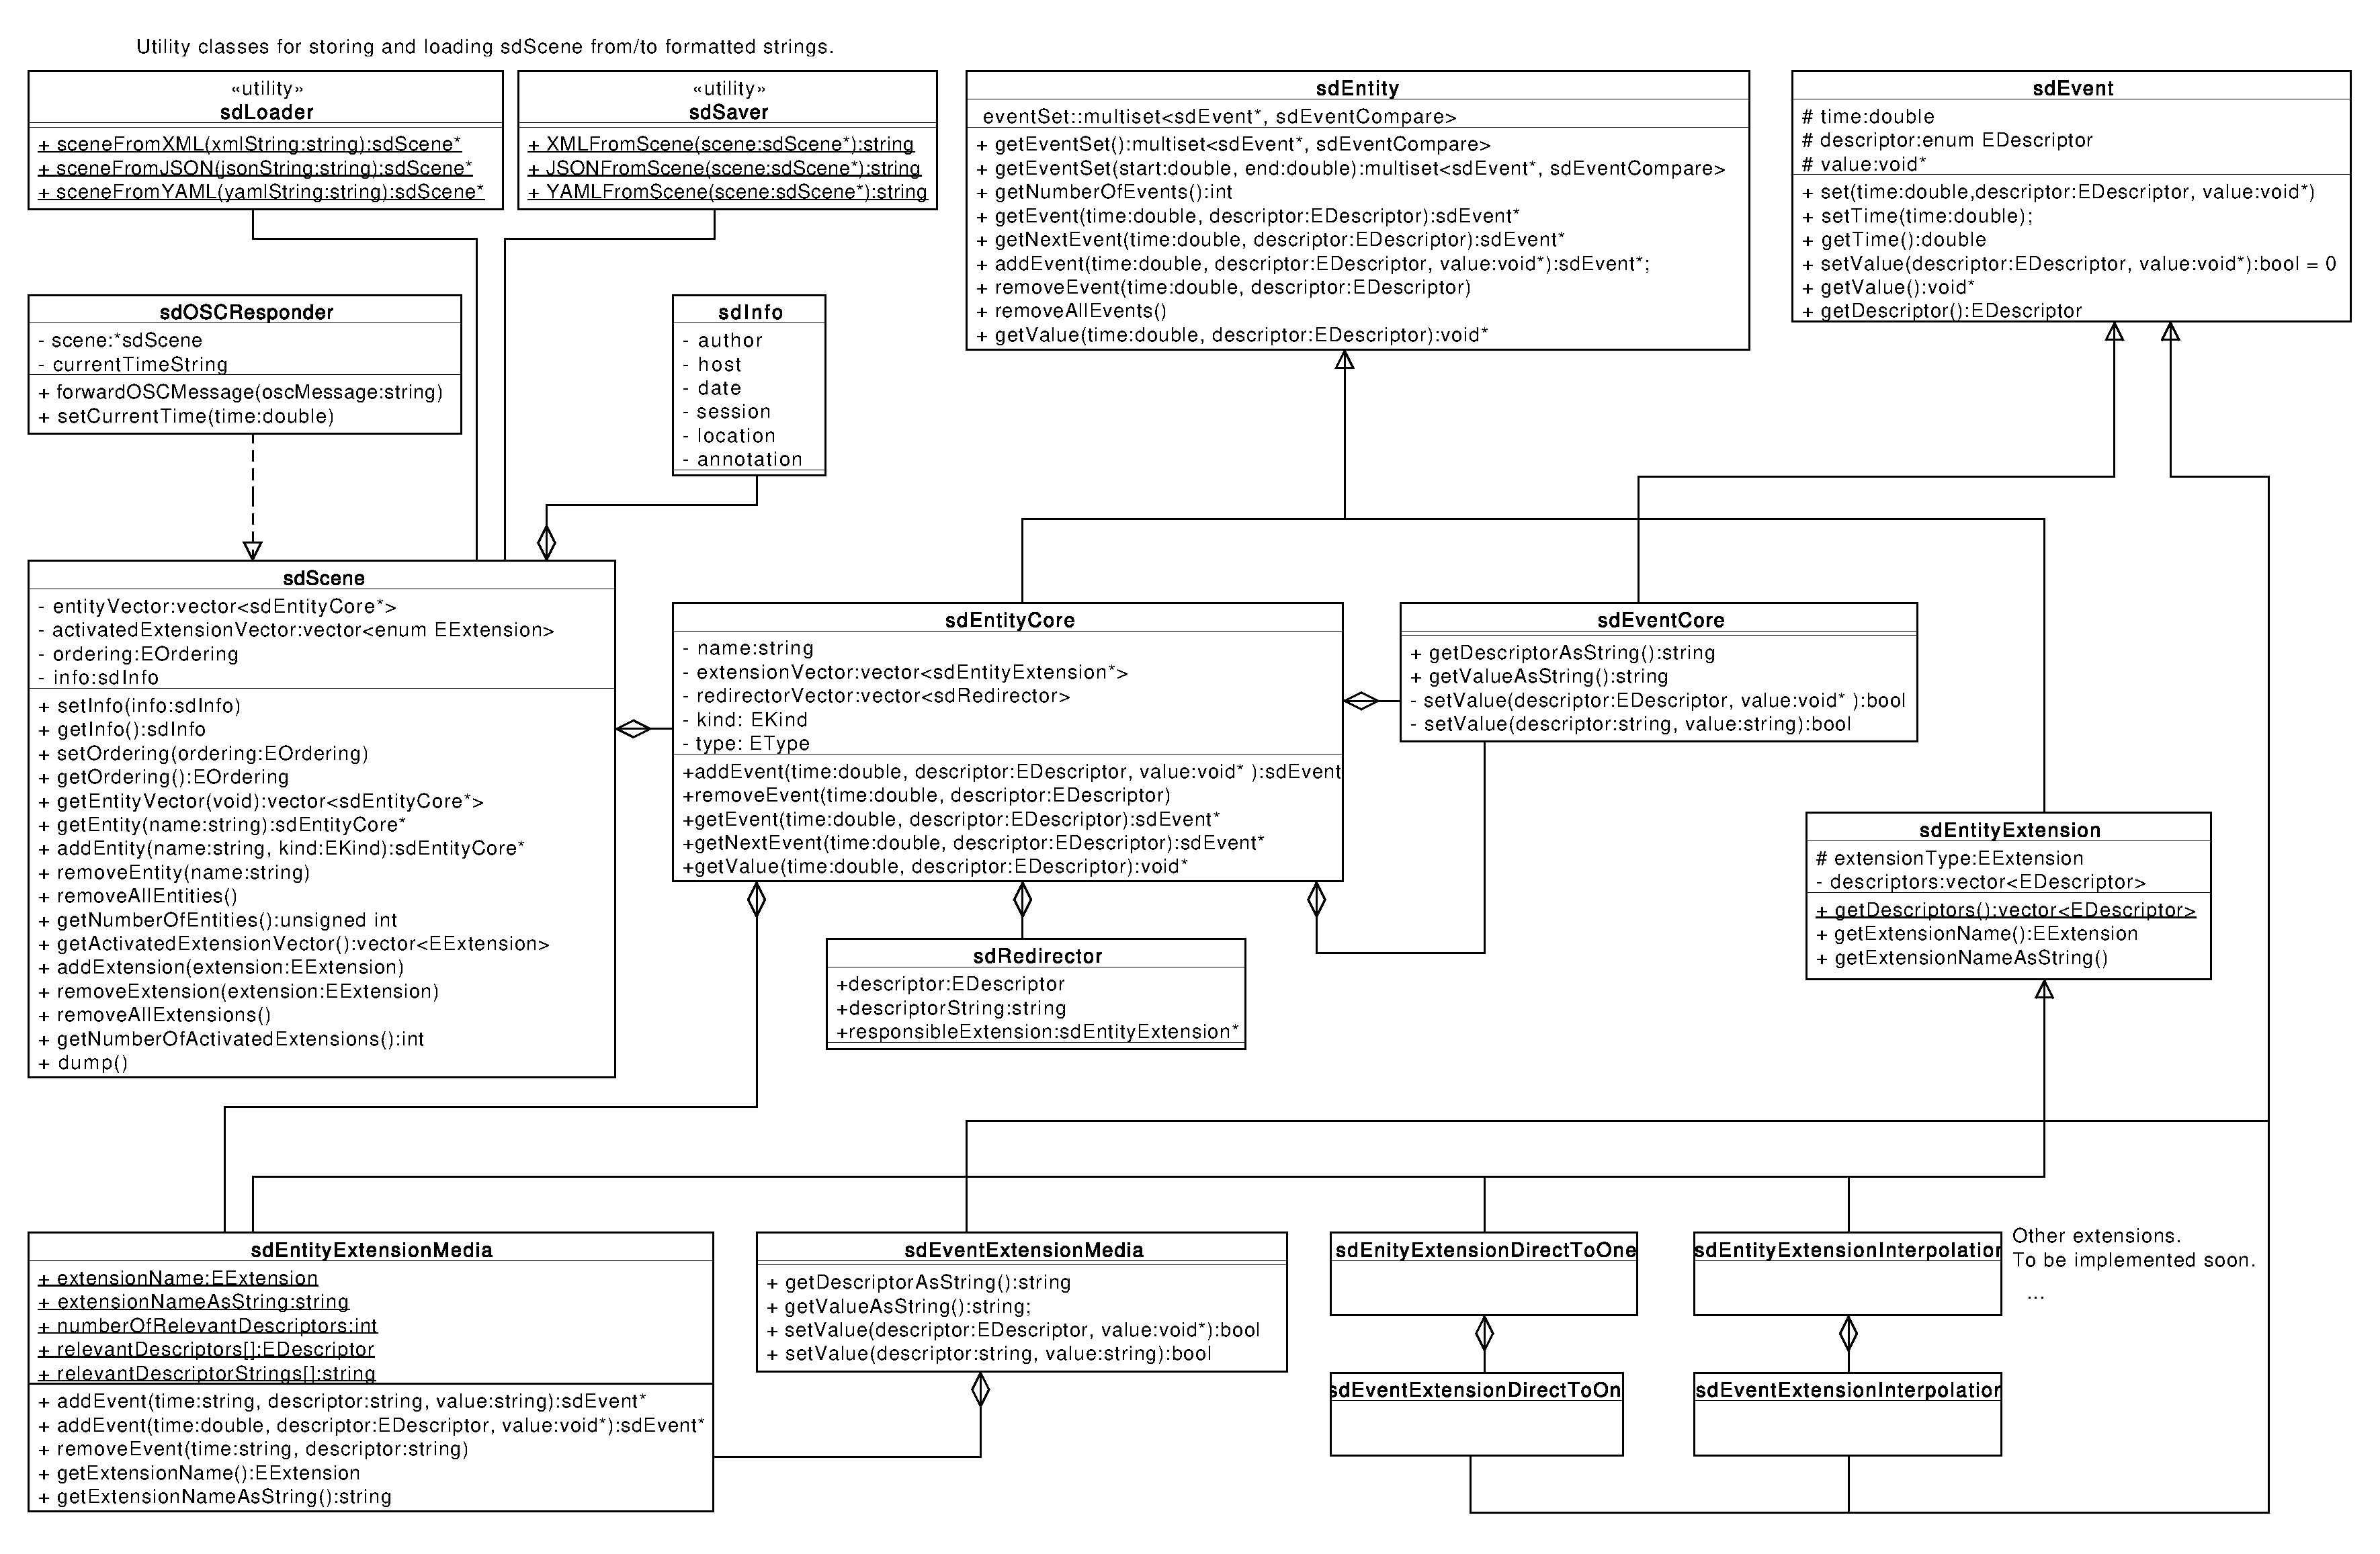
\includegraphics[width= 17.5cm]{classes.pdf}}
\caption{Class Structure}
\label{fig:class_structure}
\end{figure*}

\subsubsection{sdScene}
An instance of {\it sdScene} maintains all data associated to a SpatDIF scene. This class offers clients the following three functionalities.

\begin{itemize}[leftmargin=*]
\item[--] Addition, deletion and modification of entities in the scene
\item[--] Addition and modification of the meta data associated to the scene
\item[--] Activation and deactivation of the extensions in the scene
\end{itemize}

Once the client activates an extension in a scene, a {\it sdScene} automatically adds extended functionalities and allocates extra buffers to all existing and newly created instances of {\it sdEntityCore}. 
By deactivating an extension, {\it sdScene} removes all extended functionalities and previously allocated buffers from all existing {\it sdEntitieCores}. 
Subsequently, all data stored in the extension buffers are discarded.

\subsubsection{sdLoader/sdSaver}
These two classes provide several utility functions and enable clients to create an instance of {\it sdScene} from a XML, JSON, or YAML string and vice versa. 
In order to maintain platform independence and to achieve maximum flexibility, the library does not handle files directly; the client software is responsible for the file management. 

These functions utilise two external libraries for parsing markup formatted strings. TinyXML-2\footnote{http://www.grinninglizard.com/tinyxml, accessed Oct. 9. 2013} and libjson\footnote{http://sourceforge.net/projects/libjson, accessed Oct. 9. 2013}.

\subsubsection{sdEvent}
This is a pure abstract class of event, that maintains following three data items.

\begin{itemize}[leftmargin=*]
\item[--] time - absolute time of the event
\item[--] descriptor - type of event
\item[--] value - actual data
\end{itemize}

\subsubsection{sdEntity}
This is a pure abstract class of entity in SpatDIF scenes. Basic functionalities, such as addition, deletion, and modification of events are implemented.

\subsubsection{sdEntityCore}
An instance of {\it sdEntityCore} maintains events with SpatDIF core descriptors and has a vector to store instances of SpatDIF extensions. 
This class is also responsible for answering queries from the client conceding its events. For example, if a client asks a {\it sdEntityCore} a value of a certain descriptor at a specific time, the {\it sdEntityCore} returns value to the client. 
The client is able to raise an query about multiple events within a certain time frame and filter events by descriptors. If the client requests values of extended descriptors, a {\it sdEntityCore} forwards the query to the attached extensions stored in the internal vector.

\subsubsection{sdEntityExtension}
This is a pure abstract class of extensions. The descendants of this class. e.g. {\it sdEntityExtensionMedia} handles the events with extended descriptors. 
If a client activates an extension in a scene, each existing instance of {\it sdEntityCore} instantiates the designated subclass of {\it sdEntityExtension} and register it in its internal vector.

\subsection{Simple Code Example}
The following code listing shows how to load an XML-formatted string obtained from a SpatDIF file into an {\it sdScene} and query the entity called `insect' for the first occurrence of an event which contains a position and a media descriptor.

\vfill

\lstinputlisting[columns=fullflexible, breaklines=true, numbers=left,xleftmargin=2em,frame=none,framexleftmargin=1.5em, basicstyle=\scriptsize\ttfamily]{example_code2.cpp} 

% \pagebreak

\noindent The code produces this console-output: 
\lstinputlisting[columns=fullflexible,breaklines=true,numbers=none,basicstyle=\scriptsize\ttfamily]{code_output.txt} 

\noindent 
The following is taking place in the code example:

\begin{itemize}[leftmargin=*]
\item[--] Line 1: {\it sdLoader::sceneFromXML} static function loads a SpatDIF scene from a XML formatted string.
\item[--] Line 2: A pointer to an entity, named `insect' is obtained by scene.getEntity member function.
\item[--] Lines 3-4: The entity `insect' is requested to return a pointer to the first event with the position and media location descriptor.
\item[--] Line 6: Querying the `insect' entity for its name
\item[--] Lines 7-9: Posting the values and time of events to the console
\end{itemize}

% \subsection{Future Work}

The above-mentioned basic class hierarchy is already implemented in the library. 
The library is also able to interpret simple XML, JSON and OSC messages and is currently examined against the example renderer application, in order to further improve its performance.  
In the next phase of the project, the complete set of extensions defined in the SpatDIF specification 0.3 will be implemented and finally a C interface will be added, which should make this tool applicable to various types of software. 
%The library will be completed by the end of 2014 and released under the MIT, BSD or similar licenses. % mentioned i its own section below

\section{The Example Application}% Jasch

An example application that implements an entire workflow for the playback of SpatDIF files is being developed. The application is called a `renderer' in analogy to visual tools, because it renders audible, in a surround setup, the information contained in a SpatDIF `bundle'.
It also serves to validate the development of the library, in the sense of a complex test case that reflects real-life usage.
The implementation has to solve all the question relating to file-handling, OSC-streams, instantiating the voices of the playback engine, panning, distance cues, and the other descriptors present in the specifications 0.3.

More importantly however, it demonstrates the power and simplicity of SpatDIF by showing how one of the most common use cases is tackled.

\subsection{Scope}

In order to provide a relevant example for the application of the `SpatDIFlib', the scope of the application has been limited deliberately.
The panning algorithm is a simple spatial windowing algorithms named ``ambipanning'' \cite{Neukom:2008ambipan} that %has the advantage of being a one-step calculation (contrary to ambisonics) CHANGED:{not sure if this is an advantage, id rather remove it}, which 
is highly flexible, easy to implement, not tied to a specific number of speakers and usable without modification both in two and three dimensional spatialization situations.
The application provides a stand-alone implementation, with a basic visualization of the scene, and the possibility to play the scene on a stereo or multichannel speaker setup.
It allows to load a SpatDIF file with associated sound files and play it through a few predefined multichannel speaker layouts.
Currently two mark-up languages are supported, XML and JSON, with more to come in the future.

\subsection{Implementation details}

This application is implemented in the creative-coding environment openFrameworks\footnote{http://www.openframeworks.cc, accessed Oct. 23. 2013}, which provides a powerful C++ toolset and a thriving community.
Since it is not particularly oriented towards sound programming, the provided classes are somewhat rudimentary.
However -- and that is its strength -- many extensions exist and it is relatively easy to add new functionalities and libraries.
One of these extension-libraries that is being used for this application is libsndfile\footnote{http://www.mega-nerd.com/libsndfile, accessed Oct. 23. 2013}, which provides a powerful audio file handling toolset.
The SpatDIF-library is linked in as a dynamic library, and provides the entire data-structure and methods for handling the scene.
The renderer runs both a sonic and visual playback of the scene.
The visual representation is a bare-bones wireframe drawing of the scene in OpenGL.
Figure \ref{fig:screenshot} shows the scene of the example application.
The sound playback runs through the sound-stream interface provided by openFrameworks.
After retrieving samples from the sound files via libsndfile, panning and distance correction is applied, before the blocks of audio-samples are output.
The signal processing chain is deliberately kept simple, to provide a clear example of the implementation of such a process.

\begin{figure}[h]
\centerline{
	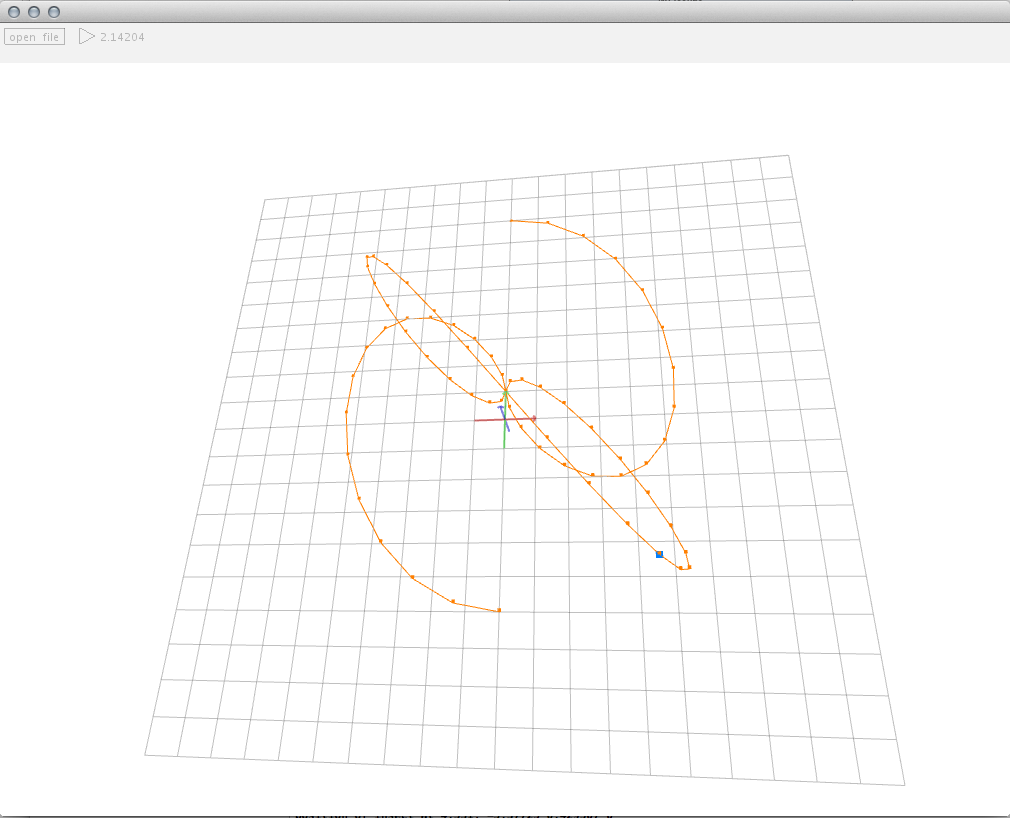
\includegraphics[width=\columnwidth]{SpatDIFrenderer_screenshot2}}
\caption{Graphical User Interface of the example renderer application, displaying the Lissajous trajectory from Chowning's `Turenas'. 
%\todo{export from OF as SVG/PDF}
}
\label{fig:screenshot}
\end{figure}

\subsection{Task Separation between SpatDIFLib and the Client Application}

The separation of labour between the library and a client application such as the example renderer presented here is very deliberate.

SpatDIFLib builds and maintains in memory the SpatDIF scene, either obtained from an already existing description stored in a file, or on the fly in real-time from elements received via OSC-formatted network packets.
It also provides an application programming interface (API) that hides most of the complexity of handling the scene data.
Two reading and two writing interfaces are planned for the library, one interfacing the file-system and the other providing the network-interface via OSC-packets.

The client application is in charge of loading the text files containing the SpatDIF-scene from the file system and handing them to the library in a text buffer.
It deals with all the audio related processes, such as loading audio files, playing them back, and configuring the audio-system.
Some of the information necessary to do this is provided by the SpatDIF scene.
In addition, the client application can open network sockets and forward OSC-formatted data to the library.
It queries the library for scene information at initialization as well as at runtime, based on its own scheduler.

\section{Availability}% Jasch

Both the library and the example application will be made freely and publicly available, as soon as the full feature-set of the 0.3 specifications are implemented and thoroughly tested.
Of course, access to the code-base can be granted on demand.

\section{Acknowledgements}% Jasch

This software development would not have been possible without the generous support of the Institute for Computer Music and Sound Technology ICST of the Zurich University of the Arts.


\printbibliography


\section{Author's Profiles}
\balance % used here in order to balance the last pages columns

\subsection*{Chikashi Miyama}
Chikashi Miyama is a composer, video artist, interface designer, performer. He received a MA (Sonology/2004) from Kunitachi College of Music, Tokyo, Japan, a Nachdiplom (Komposition im Elektronischen Studio/2007) from Music academy of Basel, Switzerland, and a Ph.D (Composition/2011) from University at Buffalo, New york, USA. His compositions have received an ICMA award (2011/UK) from the International Computer Music Association, a second prize in SEAMUS commission competition (2010/St. Cloud, USA), a special prize in Destellos Competition (2009/Argentina), and a honorable mention in the Bourges Electroacoustic Music Competition (2002/France). Several works of him are included on the DVD of the Computer Music Journal Vol.28 by MIT press, and ICMC official CD/DVD(2005/2011). In 2011, he received a research grant from DAAD (German Academic Exchange Service) and worked as a visiting researcher at ZKM, Karlsruhe, Germany. He has taught computer music at University at Buffalo, USA and College of Arts Bern, Switzerland. He is currently teaching at College of Music and Dance Cologne, College of Music Basel, and Zurich University of the Arts. http://chikashi.net

\subsection*{Jan C. Schacher}
A doublebass-player, composer and digital artist, Jan Schacher is active in electronic and exploratory music. His main focus is on works combining digital sound and images, abstract graphics and experimental video in the field of electro-acoustic music and in mixed-media projects for the stage and in installations. Jan Schacher has been invited as artist and lecturer to numerous cultural and academic institutions and has presented installations in galleries and performances in clubs and at festivals such as the Sonar Festival (Barcelona), Edinburgh Festival, the Singapore Arts Festival, the Holland Festival (Amsterdam), the Sonic Circuits Festival, Washington DC and numerous venues throughout Europe, North America, Australia and Asia. He is an associate researcher at the Zurich University of the Arts and doctoral candidate at the Royal Conservatory Antwerp.
He has published peer-reviewed articles in the context of computer music, new interfaces for musical expression as well as on the topic of artistic research.


\end{document}


